\subsection*{Partie 1. La famille d'Oedipe (\(\text{oedipe.txt}\))}\label{subsec:ss_1}
\addcontentsline{toc}{subsection}{\nameref{subsec:ss_1}}

Reprendre la base de faits d'Oedipe (le fichier \texttt{oedipe-family-facts.lp} qui vous a été fourni au TP1).
Les prédicats de la base de faits qui nous intéressent sont: 
\begin{itemize}
    \item \(\text{homme}\),
    \item \(\text{femme}\),
    \item \(\text{aEnfant}\).
    \item On n'utilisera pas le prédicat \(\text{roi}\).
\end{itemize}

Quand on vous demande de définir un prédicat, vous pouvez définir des prédicats intermédiaires.

Dans le fichier texte, donnez \defemph{toutes les règles utilisées} pour répondre aux questions.

% ----- Consignes exo 1 ----- %
\begin{td-exo}[]\,\\ % 1
    Définir le prédicat unaire \(\text{sansEnfant}(X)\) qui est vrai si \(X\) n'a pas d'enfant connu.
    Combien de faits de prédicat \(\text{sansEnfant}(X)\) obtenez-vous?
\end{td-exo}

% ----- Solutions exo 1 ----- %
\iftoggle{showsolutions}{
	\begin{td-sol}[]\,\\ % 1
        On rappelle la structure de la famille d'Oedipe:

        \vspace{0.2cm}
        \ffigbox[\FBwidth]{%
\caption{\centering La famille d'Oedipe}\label{Fig:oedipe_tree}
}{
    \fbox{
        \begin{tikzpicture}[every node/.style={font=\small}]

            % =========================
            % STYLES
            % =========================
            \tikzset{
                H/.style={text=blue},
                F/.style={text=orange!90!black},
                person/.style={align=center},
            }

            % =========================
            % NODES (COORDINATES)
            % =========================

            % Top generation - crown scaled much smaller to match \faCrown size
            \node[person,H] (Agenor) at (0,0) {Agenor \raisebox{3pt}{\scalebox{0.35}{\pgfornament{147}}}};

            % Cadmos + Harmonie
            \node[person,H] (Cadmos)   at (-2,-1.5) {Cadmos \faCrown};
            \node[person,F]        (Harmonie) at ( 2,-1.5) {Harmonie};

            % Children of Cadmos - increased spacing
            \node[person,F] (Ino)    at (-4.5,-3) {Ino};
            \node[person,F] (Agave)  at (-2,-3) {Agavé};
            \node[person,H] (Polydore) at (0,-3) {Polydore};
            \node[person,F] (Nictis) at (2,-3) {Nictéis};

            % Agave line
            \node[person,H] (Penthe)  at (-2,-4.2) {Penthée \faCrown};
            \node[person,H] (Oclosos) at (-2,-5.4) {Oclosos};
            \node[person,H] (Menecee) at (-2,-6.6) {Ménecée};

            % Children of Ménecée: Creon & Jocaste
            \node[person,H] (Creon) at (-4,-7.8) {Créon \faCrown};
            \node[person,F]           (Jocaste) at (0,-7.8) {Jocaste};

            \node[person,F] (Eurydice) at (-6,-7.8) {Eurydice};
            \node[person,H] (Hemon)    at (-4,-9.3) {Hémon};

            % Jocaste + Oedipe
            \node[person,H] (Oedipe) at (2,-7.8) {Œdipe \faCrown};

            % Children of Jocaste & Oedipe (shared) - increased spacing
            \node[person,F] (Antigone) at (0,-9.3) {Antigone};
            \node[person,F] (Ismene)   at (1.8,-9.3) {Ismène};
            \node[person,H] (Eteocle)  at (3.6,-9.3) {Étéocle \faCrown};
            \node[person,H] (Polynice) at (5.4,-9.3) {Polynice};

            % Increased spacing between Ladamos and Thersandre
            \node[person,H] (Ladamos)   at (3.6,-10.8) {Ladamos \faCrown};
            \node[person,H] (Thersandre) at (5.4,-10.8) {Thersandre};

            % Polydore line
            \node[person,H] (Labdacos) at (0,-4.2) {Labdacos};
            \node[person,H] (Laios)    at (0,-5.4) {Laïos};

            % =========================
            % CONNECTIONS (using anchor points and aligned junctions)
            % =========================

            % Agenor → Cadmos
            \draw (Agenor.south) -- (Cadmos.north);

            % Cadmos + Harmonie → children (all at same y-level)
            \coordinate (CadmosHarmonieJunction) at (0,-2.25);
            \draw (Cadmos.south) -- (Cadmos.south |- CadmosHarmonieJunction) -- (CadmosHarmonieJunction);
            \draw (Harmonie.south) -- (Harmonie.south |- CadmosHarmonieJunction) -- (CadmosHarmonieJunction);
            \draw (CadmosHarmonieJunction) -| (Ino.north);
            \draw (CadmosHarmonieJunction) -| (Agave.north);
            \draw (CadmosHarmonieJunction) -| (Polydore.north);

            % Agave line
            \draw (Agave.south) -- (Penthe.north);
            \draw (Penthe.south) -- (Oclosos.north);
            \draw (Oclosos.south) -- (Menecee.north);

            % Ménecée → Creon & Jocaste (aligned junction)
            \coordinate (MeneceeJunction) at (-2,-7.2);
            \draw (Menecee.south) -- (MeneceeJunction);
            \draw (MeneceeJunction) -| (Creon.north);
            \draw (MeneceeJunction) -| (Jocaste.north);

            % Creon + Eurydice → Hemon (aligned junction)
            \coordinate (CreonEurydiceJunction) at (-5,-8.6);
            \draw (Eurydice.south) -- (Eurydice.south |- CreonEurydiceJunction) -- (CreonEurydiceJunction);
            \draw (Creon.south) -- (Creon.south |- CreonEurydiceJunction) -- (CreonEurydiceJunction);
            \draw (CreonEurydiceJunction) -- (Hemon.north);

            % Polydore + Nictis → Labdacos (aligned junction)
            \coordinate (PolydoreNictisJunction) at (1,-3.6);
            \draw (Polydore.south) -- (Polydore.south |- PolydoreNictisJunction) -- (PolydoreNictisJunction);
            \draw (Nictis.south) -- (Nictis.south |- PolydoreNictisJunction) -- (PolydoreNictisJunction);
            \draw (PolydoreNictisJunction) -- (Labdacos.north);
            
            \draw (Labdacos.south) -- (Laios.north);

            % Laios → Oedipe
            \draw (Laios.south) -- ++(0,-0.5) -| (Oedipe.north);

            % Jocaste ↔ Oedipe (couple - horizontal line)
            \draw (Jocaste.east) -- (Oedipe.west);

            % Their children (converge at common point at same y-level)
            \coordinate (JocasteOedipeJunction) at (1,-8.6);
            \draw (Jocaste.south) -- (Jocaste.south |- JocasteOedipeJunction) -- (JocasteOedipeJunction);
            \draw (Oedipe.south) -- (Oedipe.south |- JocasteOedipeJunction) -- (JocasteOedipeJunction);
            
            \draw (JocasteOedipeJunction) -| (Antigone.north);
            \draw (JocasteOedipeJunction) -| (Ismene.north);
            \draw (JocasteOedipeJunction) -| (Eteocle.north);
            \draw (JocasteOedipeJunction) -| (Polynice.north);

            % Children of Eteocle / Polynice
            \draw (Eteocle.south) -- (Ladamos.north);
            \draw (Polynice.south) -- (Thersandre.north);

            % =========================
            % LEGEND
            % =========================
            \node[draw, thick, fill=white, align=left, font=\footnotesize, 
            inner sep=8pt, anchor=north west] at (-7,0.5) {
                \textbf{Légende :} \\[3pt]
                \textcolor{blue}{Bleu} = Homme \\[2pt]
                \textcolor{orange!90!black}{Orange} = Femme \\[2pt]
                \faCrown\ = Roi de Thèbes \\[2pt]
                \raisebox{3pt}{\scalebox{0.35}{\pgfornament{147}}} = Roi de Tyr
            };

        \end{tikzpicture}
    }
}

        \newpage

        On définit le prédicat \(\text{sansEnfant}(X)\) comme suit:

        \clingoFile{./tp_3_code/exo_1.clingo}

        En lançant Clingo, on obtient la sortie suivante:

        \clingoFile{./tp_3_code/exo_1_output.txt}
        On obtient 6 prédicats \(\text{sansEnfant}(X)\) qu'on peut facilement vérifier sur la figure~\ref{Fig:oedipe_tree}.
	\end{td-sol}
}{}

% ----- Consignes exo 2 ----- %
\begin{td-exo}[]\,\\ % 2
    Définir le prédicat unaire \(\text{aAuMoinsDeuxEnfants}(X)\) qui est vrai si \(X\) a au moins deux enfants.
    Combien de faits de prédicat \(\text{aAuMoinsDeuxEnfants}(X)\) obtenez-vous?
\end{td-exo}

% ----- Solutions exo 2 ----- %
\iftoggle{showsolutions}{
	\begin{td-sol}[]\,\\ % 2
        On définit le prédicat \(\text{aAuMoinsDeuxEnfants}(X)\) comme suit:

        \clingoFile{./tp_3_code/exo_2.clingo}

        En lançant Clingo, on obtient la sortie suivante:

        \clingoFile{./tp_3_code/exo_2_output.txt}
        On obtient 5 prédicats \(\text{aAuMoinsDeuxEnfants}(X)\) qu'on peut facilement vérifier sur la figure~\ref{Fig:oedipe_tree}.
	\end{td-sol}
}{}

% ----- Consignes exo 3 ----- %
\begin{td-exo}[]\,\\ % 3
    Définir le prédicat unaire \(\text{femmeEnfantUnique}(X)\) qui est vrai si \(X\) est une femme ayant un unique enfant.
    Combien de faits de prédicat \(\text{femmeEnfantUnique}(X)\) obtenez-vous?
\end{td-exo}

% ----- Solutions exo 3 ----- %
\iftoggle{showsolutions}{
	\begin{td-sol}[]\,\\ % 3
        On définit le prédicat \(\text{femmeEnfantUnique}(X)\) comme suit:

        \clingoFile{./tp_3_code/exo_3.clingo}

        En lançant Clingo, on obtient la sortie suivante:

        \clingoFile{./tp_3_code/exo_3_output.txt}
        On obtient 3 prédicats \(\text{femmeEnfantUnique}(X)\) qu'on peut vérifier sur la figure~\ref{Fig:oedipe_tree}.
	\end{td-sol}
}{}

% ----- Consignes exo 4 ----- %
\begin{td-exo}[]\,\\ % 4
    Définir les choses suivantes:
    \begin{itemize}
        \item le prédicat binaire \(\text{ancetre}(X,Y)\) qui est vrai si \(X\) est un ancêtre de \(Y\). On suppose ici que tout ascendant (y compris un parent) est un ancêtre et que personne n'est son propre ancêtre.
        \item le prédicat ternaire \(\text{ancetreCommun}(Z,X,Y)\) qui est vrai si \(Z\) est un ancêtre commun de \(X\) et \(Y\) (avec \(X \neq Y\)).
        \item le prédicat \(\text{answer}\) qui donne la réponse à la question \og{}Qui sont les plus lointains ancêtre communs à \defemph{Antigone} et \defemph{Laios}?\fg{} où un plus loin ancêtre commun est un ancêtre commun dont on ne connait pas de parent.
    \end{itemize}
\end{td-exo}

% ----- Solutions exo 4 ----- %
\iftoggle{showsolutions}{
	\begin{td-sol}[]\, % 4
        \begin{itemize}
            \item On définit le prédicat \(\text{ancetre}(X,Y)\) comme suit:
            \clingoFile{./tp_3_code/exo_4_ancetre.clingo}
            \item On définit le prédicat \(\text{ancetreCommun}(Z,X,Y)\) comme suit:
            \clingoFile{./tp_3_code/exo_4_ancetreCommun.clingo}
            \item On définit le prédicat \(\text{answer}\) comme suit:
            \clingoFile{./tp_3_code/exo_4_answer.clingo}
            En lançant Clingo, on obtient la sortie suivante:
            \clingoFile{./tp_3_code/exo_4_output.txt}
            La réponse est donc que les plus lointains ancêtres communs à Antigone et Laios sont:
            Nicteis, Harmonie et Agenor.
        \end{itemize}
	\end{td-sol}
}{}

Le code complet est donné en annexe~\ref{annex:code-oedipe}.







\subsection*{Partie 2. Configuration automobile (\(\text{config.txt}\))}\label{subsec:ss_2}
\addcontentsline{toc}{subsection}{\nameref{subsec:ss_2}}

On reprend le problème de configuration automobile du TP2 dont on rappelle l'énoncé ci-dessous.

Une firme automobile élabore un nouveau modèle de voiture fabriquée dans toute l'Europe:
\begin{itemize}
    \item les portières et le capot sont fabriqués à Lille où l'on ne dispose que de peinture rouge, jaune et noire;
    \item la carrosserie est faite à Hambourg où l'on a de la peinture blanche, jaune, rouge et noire;
    \item les pare-chocs, réalisés à Palerme, sont toujours blancs;
    \item la bâche du toit ouvrant, faite à Madrid, ne peut être que blanche, jaune ou rouge;
    \item les enjoliveurs sont fabriqués à Athènes où l'on a de la peinture rouge et jaune.
\end{itemize}

Le constructeur de la voiture a les exigences suivantes:
\begin{itemize}
    \item la carrosserie, les portières et le capot sont de la même couleur;
    \item les enjoliveurs, les pare-chocs et la bâche du toit ouvrant doivent être (strictement) plus clairs que la carrosserie (on considère que jaune est plus clair que rouge; blanc et noir étant les deux extrêmes).
\end{itemize}

On souhaite déterminer l'ensemble des configurations possibles pour ce modèle. On se donne le prédicat unaire \defemph{objet} et les faits suivants pour énumérer les composants de la voiture:
\clingoFile{./tp_2_code/exo_2_1.clingo}

On considère les couleurs blanc, jaune, rouge et noir, qu'on représente par les constantes \(b, j, r, n\).

% ----- Consignes exo 1 ----- %
\begin{td-exo}[]\,\\ % 1
    Rendre votre programme ASP qui répond au problème de configuration automobile complet en y ajoutant les contraintes correspondant aux exigences du constructeur.
\end{td-exo}

% ----- Solutions exo 1 ----- %
\iftoggle{showsolutions}{
    \begin{td-sol}[]\,\\ % 1
        Voir annexe~\ref{annex:code-voiture} pour le code complet.
    \end{td-sol}
}{}

% ----- Consignes exo 2 ----- %
\begin{td-exo}[]\,\\ % 2
    Pour gérer la notion de \og{}couleur plus claire\fg{} utilisant le prédicat binaire \(\text{plusClair}(X,Y)\), avez-vous introduit seulement des faits dans votre programme ou également une règle (dans ce cas, donnez cette règle)?

    Dans chaque modèle stable, combien obtenez-vous de faits ayant le prédicat \(\text{plusClair}\)?
\end{td-exo}

% ----- Solutions exo 2 ----- %
\iftoggle{showsolutions}{
    \begin{td-sol}[]\,\\ % 2
        On a introduit seulement des faits pour le prédicat \(\text{plusClair}(X,Y)\):
        \clingoFile{./tp_3_code/part2_exo2.clingo}

        On obtient 6 faits ayant le prédicat \(\text{plusClair}\) dans chaque modèle stable.
    \end{td-sol}
}{}

% ----- Consignes exo 3 ----- %
\begin{td-exo}[]\,\\ % 3
    Par quelles contraintes négatives avez-vous représenté la condition \og{}l'enjoliveur, le pare-chocs et la bâche sont plus clairs que la carrosserie\fg{}?
\end{td-exo}

% ----- Solutions exo 3 ----- %
\iftoggle{showsolutions}{
    \begin{td-sol}[]\,\\ % 3
        On a utilisé les contraintes négatives suivantes:
        \clingoFile{./tp_3_code/part2_exo3.clingo}
    \end{td-sol}
}{}

% ----- Consignes exo 4 ----- %
\begin{td-exo}[]\,\\ % 4
    Vous semble-t-il possible d'écrire la condition de la question précédente sous forme de règles positives? Expliquez (donnez les règles positives qui remplaçent les contraintes négatives si vous pensez que c'est possible et sinon expliquez pourquoi ce n'est pas possible).
\end{td-exo}

% ----- Solutions exo 4 ----- %
\iftoggle{showsolutions}{
    \begin{td-sol}[]\,\\ % 4
        En utilisant des conditions négatives on retire des configurations interdites à l'ensemble des configurations possibles, qu'on a généré au début. Si on ne change pas cette partie au début il restera toujours des configurations interdites.

        On peut utiliser des règles positives pour générer uniquement des configurations valides, mais dans ce cas il faut réécrire toute la partie de génération des configurations possibles au début.
    \end{td-sol}
}{}







\subsection*{Partie 3. Modélisation d'un autre problème de satisfaction de contraintes (\(\text{table.txt}\))}\label{subsec:ss_3}
\addcontentsline{toc}{subsection}{\nameref{subsec:ss_3}}

On considère le problème suivant:

Il y a 6 sièges autour d'une table ronde et 6 invités à placer sur ces sièges. Le but est de trouver toutes les façons d'affecter un siège à un invité sachant qu'il faut respecter certaines contraintes liées aux relations de sympathie ou antipathie entre les invités.

Voici un squelette de programme ASP dans lequel on utilise deux prédicats: \(\text{guest}(X)\) pour dire que \(X\) est un invité et \(\text{at}(X,Y)\) pour dire que \(X\) est placé au siège \(Y\).

On utilise aussi la règle du choix comme raccourci pour éviter d'avoir 6 règles disant que tout invité a un siège parmi les 6 (prenez cette règle telle quelle, vous n'aurez pas à la modifier):

\clingoFile{./tp_3_code/table_squelette.clingo}

% ----- Consignes exo 1 ----- %
\begin{td-exo}[]\,\\ % 1
    Ajouter une contrainte exprimant qu'une place ne peut pas recevoir deux invités.
\end{td-exo}

% ----- Solutions exo 1 ----- %
\iftoggle{showsolutions}{
    \begin{td-sol}[]\,\\ % 1
        On ajoute la contrainte suivante:
        \clingoFile{./tp_3_code/part3_exo1.clingo}
    \end{td-sol}
}{}

% ----- Consignes exo 2 ----- %
\begin{td-exo}[]\,\\ % 2
    Par quelle formule définir le nombre de modèles stables à cette étape? (Vous pouvez aussi donner le nombre de modèles stables mais l'important est de donner la formule qui permet de le calculer.)
\end{td-exo}

% ----- Solutions exo 2 ----- %
\iftoggle{showsolutions}{
    \begin{td-sol}[]\,\\ % 2
        Le nombre de modèles stables est donné par la formule \(6!\) soit \(720\). % chktex 40
        Elle vient du fait que le premier invité pour choisir n'importe laquelle des 6 places de départ, le suivant n'a plus que 5 places possibles, le suivant 4, etc.
    \end{td-sol}
}{}

% ----- Consignes exo 3 ----- %
\begin{td-exo}[]\,\\ % 3
    Définir la notion de \og{}côte à côte\fg{} grâce au prédicat binaire \(\text{nextTo}(X,Y)\) qui est vrai si \(X\) et \(Y\) ont des places adjacentes autour de la table, qui, rappelons-le, est ronde (ainsi les places 1 et 6 sont adjacentes).

    \textbf{Conseil}: faites simple pour commencer et vous pourrez faire plus élégant si vous en avez le temps à la fin de l'exercice.
\end{td-exo}

% ----- Solutions exo 3 ----- %
\iftoggle{showsolutions}{
    \begin{td-sol}[]\,\\ % 3
        On définit le prédicat \(\text{nextTo}(X,Y)\) comme suit:
        \clingoFile{./tp_3_code/part3_exo3.clingo}

        On gère initialement les cas simples de gauche et droite, puis on ajoute les cas particuliers des extrémités 1 et 6.
    \end{td-sol}
}{}

% ----- Consignes exo 4 ----- %
\begin{td-exo}[]\,\\ % 4
    On gère maintenant deux contraintes de placement:
    \begin{enumerate}
        \item Certains invités s'apprécient particulièrement (prédicat binaire \(\text{like}(X,Y)\)) et on veut vraiment les placer côte à côte.
        \item D'autres invités ne s'apprécient pas du tout (prédicat binaire \(\text{dislike}(X,Y)\)) et on veut absolument éviter de les placer côte à côte.
    \end{enumerate}
    On a ainsi les faits suivants:
    \clingoFile{./tp_3_code/part3_exo4_faits.clingo}
    Ajouter à votre programme les contraintes de placement correspondantes.
    Combien de solutions obtenez-vous?
\end{td-exo}

% ----- Solutions exo 4 ----- %
\iftoggle{showsolutions}{
    \begin{td-sol}[]\,\\ % 4
        On ajoute les contraintes suivantes:
        \clingoFile{./tp_3_code/part3_exo4_contraintes.clingo}

        En lançant Clingo, on obtient 96 solutions respectant les contraintes de placement.
    \end{td-sol}
}{}

Le code complet est donné en annexe~\ref{annex:code-csp}.




\subsection*{Partie 4. Configuration auomobile 2 (\(\text{config2.txt}\))}\label{subsec:ss_4}
\addcontentsline{toc}{subsection}{\nameref{subsec:ss_4}}

On reprend le problème de configuration automobile. Dans le TP, on vous demandait de gérer les domaines sous forme de contraintes négatives qui interdisent certaines couleurs selon les composants d'une voiture. On vous demande maintenant une deuxième version du programme où les domaines sont donnés sous forme de faits en utilisant un prédicat binaire \(\text{aColPossible}(X,Y)\) qui dit que \(X\) a pour couleur possible \(Y\). Par exemple, pour les portières on aurait:
\clingoFile{./tp_3_code/part4_exemple.clingo}

Dans un fichier texte nommé \texttt{config2.txt}, donner une autre version des règles qui génèrent toutes les affectations de façon à pouvoir supprimer les contraintes négatives qui interdisaient aux composants d'avoir des couleurs hors de leur domaine. Obtenez-vous un résultat satisfaisant?

% ----- Solutions exo 1 ----- %
\iftoggle{showsolutions}{
    \begin{td-sol}[]\,\\ % 1
        Voir annexe~\ref{annex:code-voiture2} pour le code complet.

        Le résultat est satisfaisant, on obtient le même nombre de configurations possibles que dans la première version du programme à condition encore une fois de modifier la partie de génération des configurations possibles.
    \end{td-sol}
}{}